\documentclass[../../main.tex]{subfiles}

\begin{document}

\label{sec:abbildungen_verkettung}

Abbildungen übersetzen Argumente, die aus ihrer Definitionsmenge kommen, in ihr jeweiliges Bild. Auf diese Weise erhält man bei einer Abbildung $f\colon U\rightarrow V$ Bilder aus der Menge $V$. Wie im folgenden Beispiel kommt es manchmal vor, dass nach Anwendung einer Abbildung direkt eine zweite Abbildung angewandt werden soll.

\begin{example}{}
    \parpic[r]{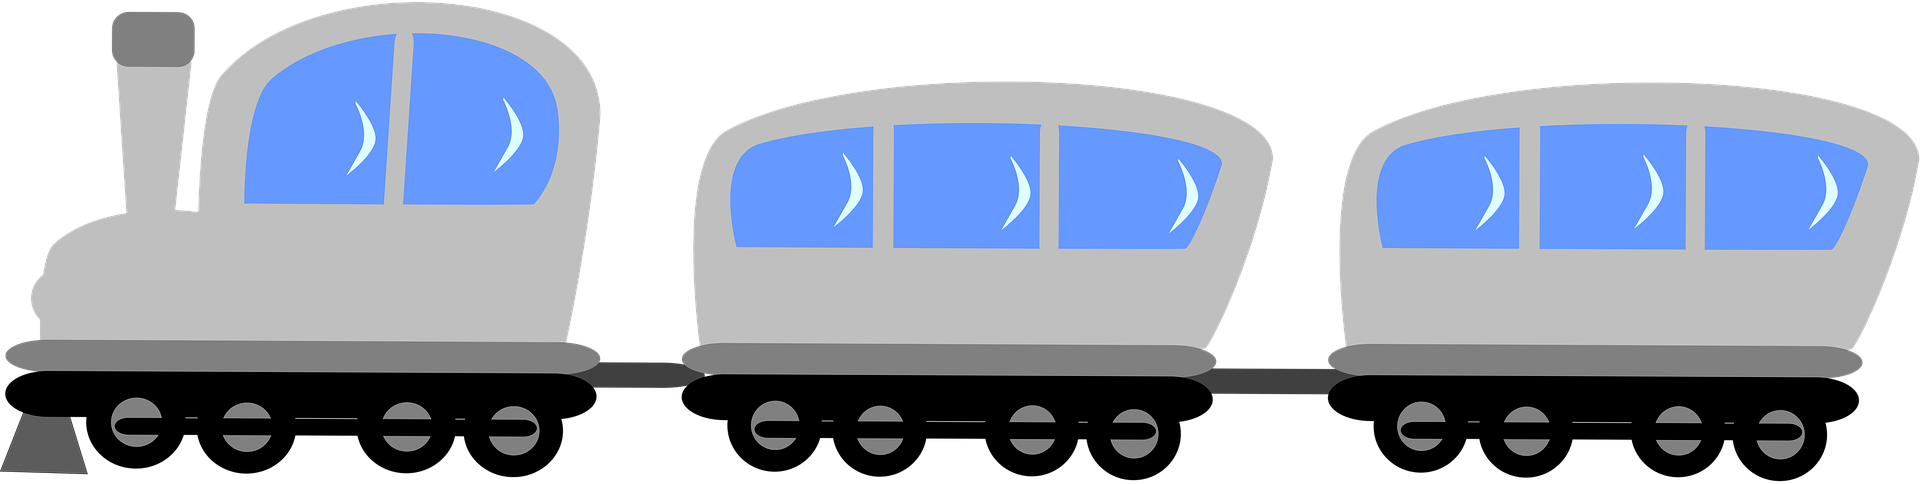
\includegraphics[width=.33\textwidth]{images/train.png}}
    Eine Gruppe von sechs Freunden möchte sich in Hamburg-Niendorf treffen. Zwei von ihnen wohnen außerhalb von Hamburg. Deswegen steigen sie zunächst in einen Zug, der sie zum Hamburger Hauptbahnhof fährt. Nach der Ankunft steigen die beiden um und fahren mit der U-Bahn weiter, bis sie ihre Freunde im Stadtteil Niendorf treffen.
    
    \picskip{0}
    Der Zug transportiert alle, die bis zur Endstation fahren, zum Hauptbahnhof (und beschreibt auf diese Weise eine Abbildung $\textsc{ZugNachHamburg}$, die alle Orte, an denen Gäste einsteigen, auf den Ort \emph{Hamburg Hbf.} abbildet). Die Straßenbahn nach Niendorf transport die beiden Freunde vom Hauptbahnhof nach Niendorf (also beschreibt sie eine Abbildung $\textsc{BahnNachNiendorf}$, die den Ort \emph{Hamburg Hbf.} auf \emph{Niendorf} abbildet).
    
    Wenn einer der Freunde in Itzehoe (einer Stadt nördlich von Hamburg) in den Zug nach Hamburg steigt und dann in die U-Bahn, dann gelangt er nach Niendorf. Auf seinen Ausgangsort \emph{Itzehoe} hat er erst die Abbildung $\textsc{ZugNachHamburg}$ angewandt ($\textsc{ZugNachHamburg}(\emph{Itzehoe})=\emph{Hamburg Hbf.}$) und anschließend durch das Einsteigen in die Straßenbahn die Abbildung $\textsc{BahnNachNiendorf}$ genutzt, um nach Niendorf zu kommen ($\textsc{BahnNachNiendorf}(\emph{Hamburg Hbf.})=\emph{Niendorf}$).
\end{example}

Bei der \textbf{Verkettung} (auch \emph{Hintereinanderausführung} oder \emph{Komposition}) von Abbildungen geht es darum, ein Argument mithilfe einer Abbildung auf sein Bild abzubilden (so, wie du das bereits aus den letzten Abschnitten kennst) und anschließend das erhaltene Bild direkt in eine zweite Abbildung einzusetzen und erneut abzubilden. Auf diese Weise wird jedes Element aus der Definitionsmenge der ersten Abbildung -- mit einem Zwischenschritt -- auf ein Element aus der Bildmenge der zweiten Abbildung abgebildet.

\begin{example}{}
    Der Freund, der aus Itzehoe nach Niendorf gefahren ist, hat zwei Abbildungen hintereinander ausgeführt, also verkettet. Er ist erst mit dem Zug nach Hamburg gefahren und anschließend mit der U-Bahn zu seinem Ziel in Niendorf. Mathematisch aufgeschrieben gilt \[\textsc{BahnNachNiendorf}(\colorbrace{\textsc{ZugNachHamburg}(\emph{Itzehoe})}{\emph{Hamburg Hbf.}})=\emph{Niendorf}.\]
\end{example}

Mathematisch funktioniert die Verkettung von Abbildungen so, dass man ein Argument $x$ zunächst benutzt, um $f(x)$ zu berechnen, d.h. um es mithilfe von $f$ abzubilden. Anschließend setzt man dieses Ergebnis in eine Abbildung $g$ ein. Man berechnet also $g(f(x))$. $f(x)$ wird an dieser Stelle als Argument für $g$ verwendet.

Zwei Abbildungen zu verketten, klappt nur dann, wenn die zweite Abbildung etwas mit den Ergebnissen der ersten anfangen kann (also für sie definiert ist). Im folgenden Bild siehst du, wie die zweite Abbildung genau dort ansetzt, wo die erste aufhört. Neben das Abbildungsdiagramm der ersten Abbildung wird ein zweites Abbildungsdiagramm gezeichnet. Dabei teilen sich beide Abbildungen eine Menge: Die zweite Abbildung nutzt die Bildmenge der ersten als ihre Definitionsmenge.

\begin{figure}[h!]
    \centering
    \begin{tikzpicture}[scale=.75]
    \draw[grayset] (-1.5,0) ellipse (0.7cm and 2cm);
    \draw[grayset] (1.5,0) ellipse (0.7cm and 2cm);
    \draw[grayset] (4.5,0) ellipse (0.7cm and 2cm);

    \node[red] (x1) at (-1.5,0.7) {$\bullet$};
    \node (x2) at (-1.5,-0.2) {$\bullet$};
    \node (x3) at (-1.5,-1.1) {$\bullet$};
    \node (y1) at (1.5,0.7) {$\bullet$};
    \node (y2) at (1.5,-0.2) {$\bullet$};
    \node[violet] (y3) at (1.5,-1.2) {$\bullet$};
    \node (z1) at (4.5,1.2) {$\bullet$};
    \node (z2) at (4.5,0.4) {$\bullet$};
    \node (z3) at (4.5,-0.4) {$\bullet$};
    \node[blue] (z4) at (4.5,-1.2) {$\bullet$};

    \draw[->] (x1) -- (y3);
    \draw[->] (x2) to[bend right] (y1);
    \draw[->] (x3) to[bend right] (y2);
    
    \draw[->] (y1) -- (z3);
    \draw[->] (y2) -- (z1);
    \draw[->] (y3) -- (z4);
    
    \node at (0,1) {$f$};
    \node at (3,1) {$g$};
\end{tikzpicture}
    \caption{Ein Element der links dargestellten Menge kann mit der eingezeichneten Abbildung $f$ in ein Element der mittleren Menge übersetzt werden (z.B. kann das rote auf das violette Element abgebildet werden). Das violette Element kann mithilfe der zweiten eingezeichneten Abbildung $g$ auf ein Element der rechten Menge abgebildet werden, und zwar auf das blaue. Das heißt, dass das rote Element insgesamt mit einem Zwischenschritt auf das blaue abgebildet wird, wenn man erst die linke und dann die rechte Abbildung anwendet. Dafür hat man zunächst $f(x)$ berechnet und das Ergebnis anschließend in die Abbildung $g$ eingesetzt, also $g(f(x))$ berechnet.}
\end{figure}

So ist es möglich, dass -- wie an einem Fließband in einer Fabrik -- erst die Abbildung $f$ ein Argument erhält und es in ein Bild übersetzt, mit dem $g$ weiterarbeiten kann. Anschließend erhält $g$ dieses Bild und verarbeitet es seinerseits weiter.

\begin{example}{}
    \parpic[r]{
        \begin{tikzpicture}
            \draw[black!25,fill=black!10] (-1.5,0) circle[radius=6mm];
            \draw[black!25,fill=black!10] (0,0) circle[radius=6mm];
            \draw[black!25,fill=black!10] (1.5,0) circle[radius=6mm];
            %node content
            \node[yellow!70!black] at (-1.5,0) {\euro};
            \node[yellow!70!black] at (0,0) {\$};
            \node[yellow!70!black] at (1.5,0) {
\includegraphics[height=10mm]{images/statue_of_liberty.png}};
            %connection lines
            \draw[very thick,black!40,->] (-1.5,0.6) to[bend left] (0,0.6);
            \draw[very thick,black!40,->] (0,-0.6) to[bend right] (1.5,-0.6);
        \end{tikzpicture}
    }
    Bei einer Reise in die USA, in denen man mit der Währung Dollar bezahlt, kann man als Europäer natürlich nicht mit Euro bezahlen. Wer dorthin reist, wechselt deshalb vorher etwas Geld, das er für die Reise einplant, in Dollar.
    \picskip{2}
    
    Mit diesem Geld ist es anschließend unter anderem möglich, vor Ort Essen in Restaurants zu kaufen sowie den Eintritt zu Sehenswürdigkeiten und anderen Touristenattraktionen zu bezahlen. Wir gehen nun davon aus, dass von dem Geld Tickets für den Besuch der Freiheitsstatue gekauft werden sollen (Preis: 40\,\$).
    
    Für einen USA-Urlaub wechselt man also erst seine Euro in Dollar und anschließend die Dollar in Eintrittskarten, Verpflegung und ähnliches. Wir wissen bereits, dass sich das Wechseln von Euro in Dollar als eine Abbildung beschreiben lässt. Angenommen, der Wechselkurs liegt bei $1.2\:\$$, die man pro Euro bekommt. Dann ordnet die Abbildung $\textsc{Dollar}\colon\Real\rightarrow\Real$ mit der Abbildungsvorschrift $\textsc{Dollar}(x)=1.2x$ dem investierten Betrag in Euro zu, wie viele Dollar man dafür erhält. Es gilt beispielsweise $\textsc{Dollar}(5)=6$, weil man 6 Dollar für 5 Euro erhalten würde.
    
    Die Abbildung $\textsc{TicketsFürDollar}\colon\Real\rightarrow\Integer$ könnte nun beschreiben, wie viele Tickets man für einen bestimmten Betrag (in Dollar) kaufen kann.
    
    Möchte man nun wissen, wie viele Tickets für die Freiheitsstatue für 100\,€ erhältlich sind, muss man diesen Betrag zunächst in Dollar umrechnen (mithilfe der Abbildung $\textsc{Dollar}$). Es gilt $\textsc{Dollar}(100)=120$. Anschließend verrät die Abbildung $\textsc{TicketsFürDollar}$, dass man $3$ Tickets kaufen kann, weil man die eben erhaltene $120$ einsetzt und $\textsc{TicketsFürDollar}(120)=3$ gilt.
    
    Wir haben erst $\textsc{Dollar}(100)$ und dann $\textsc{TicketsFürDollar}(120)$ berechnet. Die $120$ ist genau das Ergebnis von $\textsc{Dollar}(100)$. Also ist \[\textsc{TicketsFürDollar}(120)=\textsc{TicketsFürDollar}(\colorbrace{\textsc{Dollar}(100)}{=120}).\]
    
    Um zu berechnen, wie viele Tickets wir für $x$ Euro bekommen, berechnen wir also $\textsc{TicketsFürDollar}(\textsc{Dollar}(x))$.
\end{example}

Zwei Abbildungen $f$ und $g$ nacheinander anzuwenden, kann sich manchmal als sinnvoll erweisen, wenn man mit einfachen Zwischenschritten zu einem bestimmten Ergebnis kommt, statt eine kompliziertere Abbildung in einem Schritt zu berechnen.

\begin{example}{}
    Wenn man im Kopf für eine bestimmte Zahl $x$ den Wert $3x+2$ ausrechnen möchte, dann kann man das nicht sinnvoll in einem Schritt tun. Stattdessen wirst du dir erst überlegen, was $3x$ ist. Anschließend wirst du $2$ zum Ergebnis addieren. In einem ersten Schritt berechnest du also die Abbildung $f(x)=3x$, die die Addition von $2$ zunächst ignoriert.
    
    Nachdem du weißt, welchen Wert $3x$ hat, addierst du darauf $2$. Mit der Abbildung $g(x)=x+2$ tust du genau das. Führst du beide Abbildungen hintereinander aus, berechnest du \[g(f(x))=g(3x)=3x+2,\] also genau das, was du berechnen wolltest -- nur mit einem Zwischenschritt.
    
    Für $x=5$ gilt zum Beispiel $f(5)=3\cdot 5=15$ und $g(f(5))=g(15)=15+2=17$. Natürlich ist auch \[\colorbrace{\colorobrace{3\cdot 5}{f(5)}+2}{g(f(5))}=17.\]
\end{example}

Gerade im letzten Beispiel hat man gesehen, dass auch die Verkettung von zwei Abbildungen selbst wieder eine Abbildung ist. Jedes Argument für $f$ wird eindeutig erst auf ein Argument für $g$ und dann auf das Bild, das $g$ produziert, abgebildet. Die Abbildung $g(f(x))$ kann daher selbst als eine Abbildung definiert werden. Sie wird die \textbf{Verkettung} oder die \textbf{Komposition} von $f$ und $g$ genannt.

\begin{definition}{Verkettung von Abbildungen}
    Es seien $U,V,W$ Mengen und $f\colon U\rightarrow V$ sowie $g\colon V\rightarrow W$ Abbildungen.
    
    Die Abbildung $g\circ f\colon U\rightarrow W$ mit \[x\mapsto (g\circ f)(x)\coloneqq g(f(x))\] heißt die \textbf{Komposition} oder \textbf{Verkettung} von $f$ und $g$.
\end{definition}

Die Abbildung $g\circ f$ bildet ihre Argumente auf das Bild ab, das man erhält, wenn man erst $f$ und dann $g$ anwendet. Hierbei sollte man sich nicht davon verwirren lassen, dass das $g$ links steht -- das $f$ wird trotzdem zuerst angewandt, denn es befindet sich bei der Schreibweise $g(f(x))$ innen. Die Schreibweise $g\circ f$ aus dieser Definition kann man als \enquote{$g$ Kringel $f$} lesen.

Die Reihenfolge, in der man $f$ und $g$ anwendet, ist für Verkettungen sehr wichtig. Einerseits kann es sein, dass man, wenn man erst $g$ anwendet, überhaupt kein Bild erhält, das in der Definitionsmenge von $f$ liegt. Es ist aber auch selbst dann, wenn die Definitions- und Bildmengen dennoch zu einander passen, nicht egal, in welcher Reihenfolge man die Abbildungen anwendet (wie im nächsten Beispiel zu sehen ist).

\begin{example}{}
    Im letzten Beispiel haben wir gesehen, dass $g(f(x))=3x+2$ ist. Die Verkettung dieser beiden Abbildungen $g\circ f$ ist die Abbildung $(g\circ f)(x)=3x+2$.
    
    Es gilt hingegen aber $(f\circ g)(x)=f(g(x))=f(x+2)=3(x+2)=3x+6$. Die Reihenfolge, in der man $f$ und $g$ anwendet, ist also sehr wichtig und verändert die Abbildung, die man bei der Verkettung erhält.
\end{example}

\begin{nutshell}{Verkettung von Abbildungen}
    \parpic[r]{\begin{tikzpicture}[scale=.6]
    \draw[grayset] (-1.5,0) ellipse (0.7cm and 2cm);
    \draw[grayset] (1.5,0) ellipse (0.7cm and 2cm);
    \draw[grayset] (4.5,0) ellipse (0.7cm and 2cm);

    \node (x1) at (-1.5,0.7) {$\bullet$};
    \node (x2) at (-1.5,-0.2) {$\bullet$};
    \node (x3) at (-1.5,-1.1) {$\bullet$};
    \node (y1) at (1.5,0.7) {$\bullet$};
    \node (y2) at (1.5,-0.2) {$\bullet$};
    \node (y3) at (1.5,-1.2) {$\bullet$};
    \node (z1) at (4.5,1.2) {$\bullet$};
    \node (z2) at (4.5,0.4) {$\bullet$};
    \node (z3) at (4.5,-0.4) {$\bullet$};
    \node (z4) at (4.5,-1.2) {$\bullet$};

    \draw[->] (x1) -- (y3);
    \draw[->] (x2) to[bend right] (y1);
    \draw[->] (x3) to[bend right] (y2);
    
    \draw[->] (y1) -- (z3);
    \draw[->] (y2) -- (z1);
    \draw[->] (y3) -- (z4);
    
    \node at (0,1) {$f$};
    \node at (3,1) {$g$};
\end{tikzpicture}}
    Zwei Abbildungen $f$ und $g$, bei denen $f$ seine Argumente in die Definitionsmenge von $g$ abbildet, können hintereinander angewandt werden. Dafür bildet man ein Element $x$ der Definitionsmenge von $f$ erst mit $f$ und das Ergebnis $f(x)$ dann mit $g$ ab. Man berechnet also $g(f(x))$.
      
    \picskip{0} 
    Die Abbildung, die jedes Element aus der Definitionsmenge von $f$ auf das Element der Bildmenge von $g$ abbildet, das man erhält, wenn man erst $f$ und dann $g$ anwendet, heißt \textbf{Verkettung} von $f$ und $g$. Sie wird geschrieben als $g\circ f$. Es gilt also $(g\circ f)(x)=g(f(x))$.
\end{nutshell}

\end{document}